\documentclass[12pt]{article}
\usepackage[utf8]{inputenc}
\usepackage[a4paper, total={6in, 10in}]{geometry}
\usepackage{graphicx} % Required for inserting images
\usepackage[italian]{babel}
\usepackage{float}
\usepackage[table]{xcolor}
\usepackage{tabularx}
\usepackage{hyperref}
\usepackage{listings}
\usepackage{color}
\usepackage{tcolorbox}

\title{Dealership ``Elite" Data Base}
\author{Elvis Perlika}
\date{\today}

\begin{document} 

\maketitle

\vspace{0.8in}

\begin{center}
    \centering
    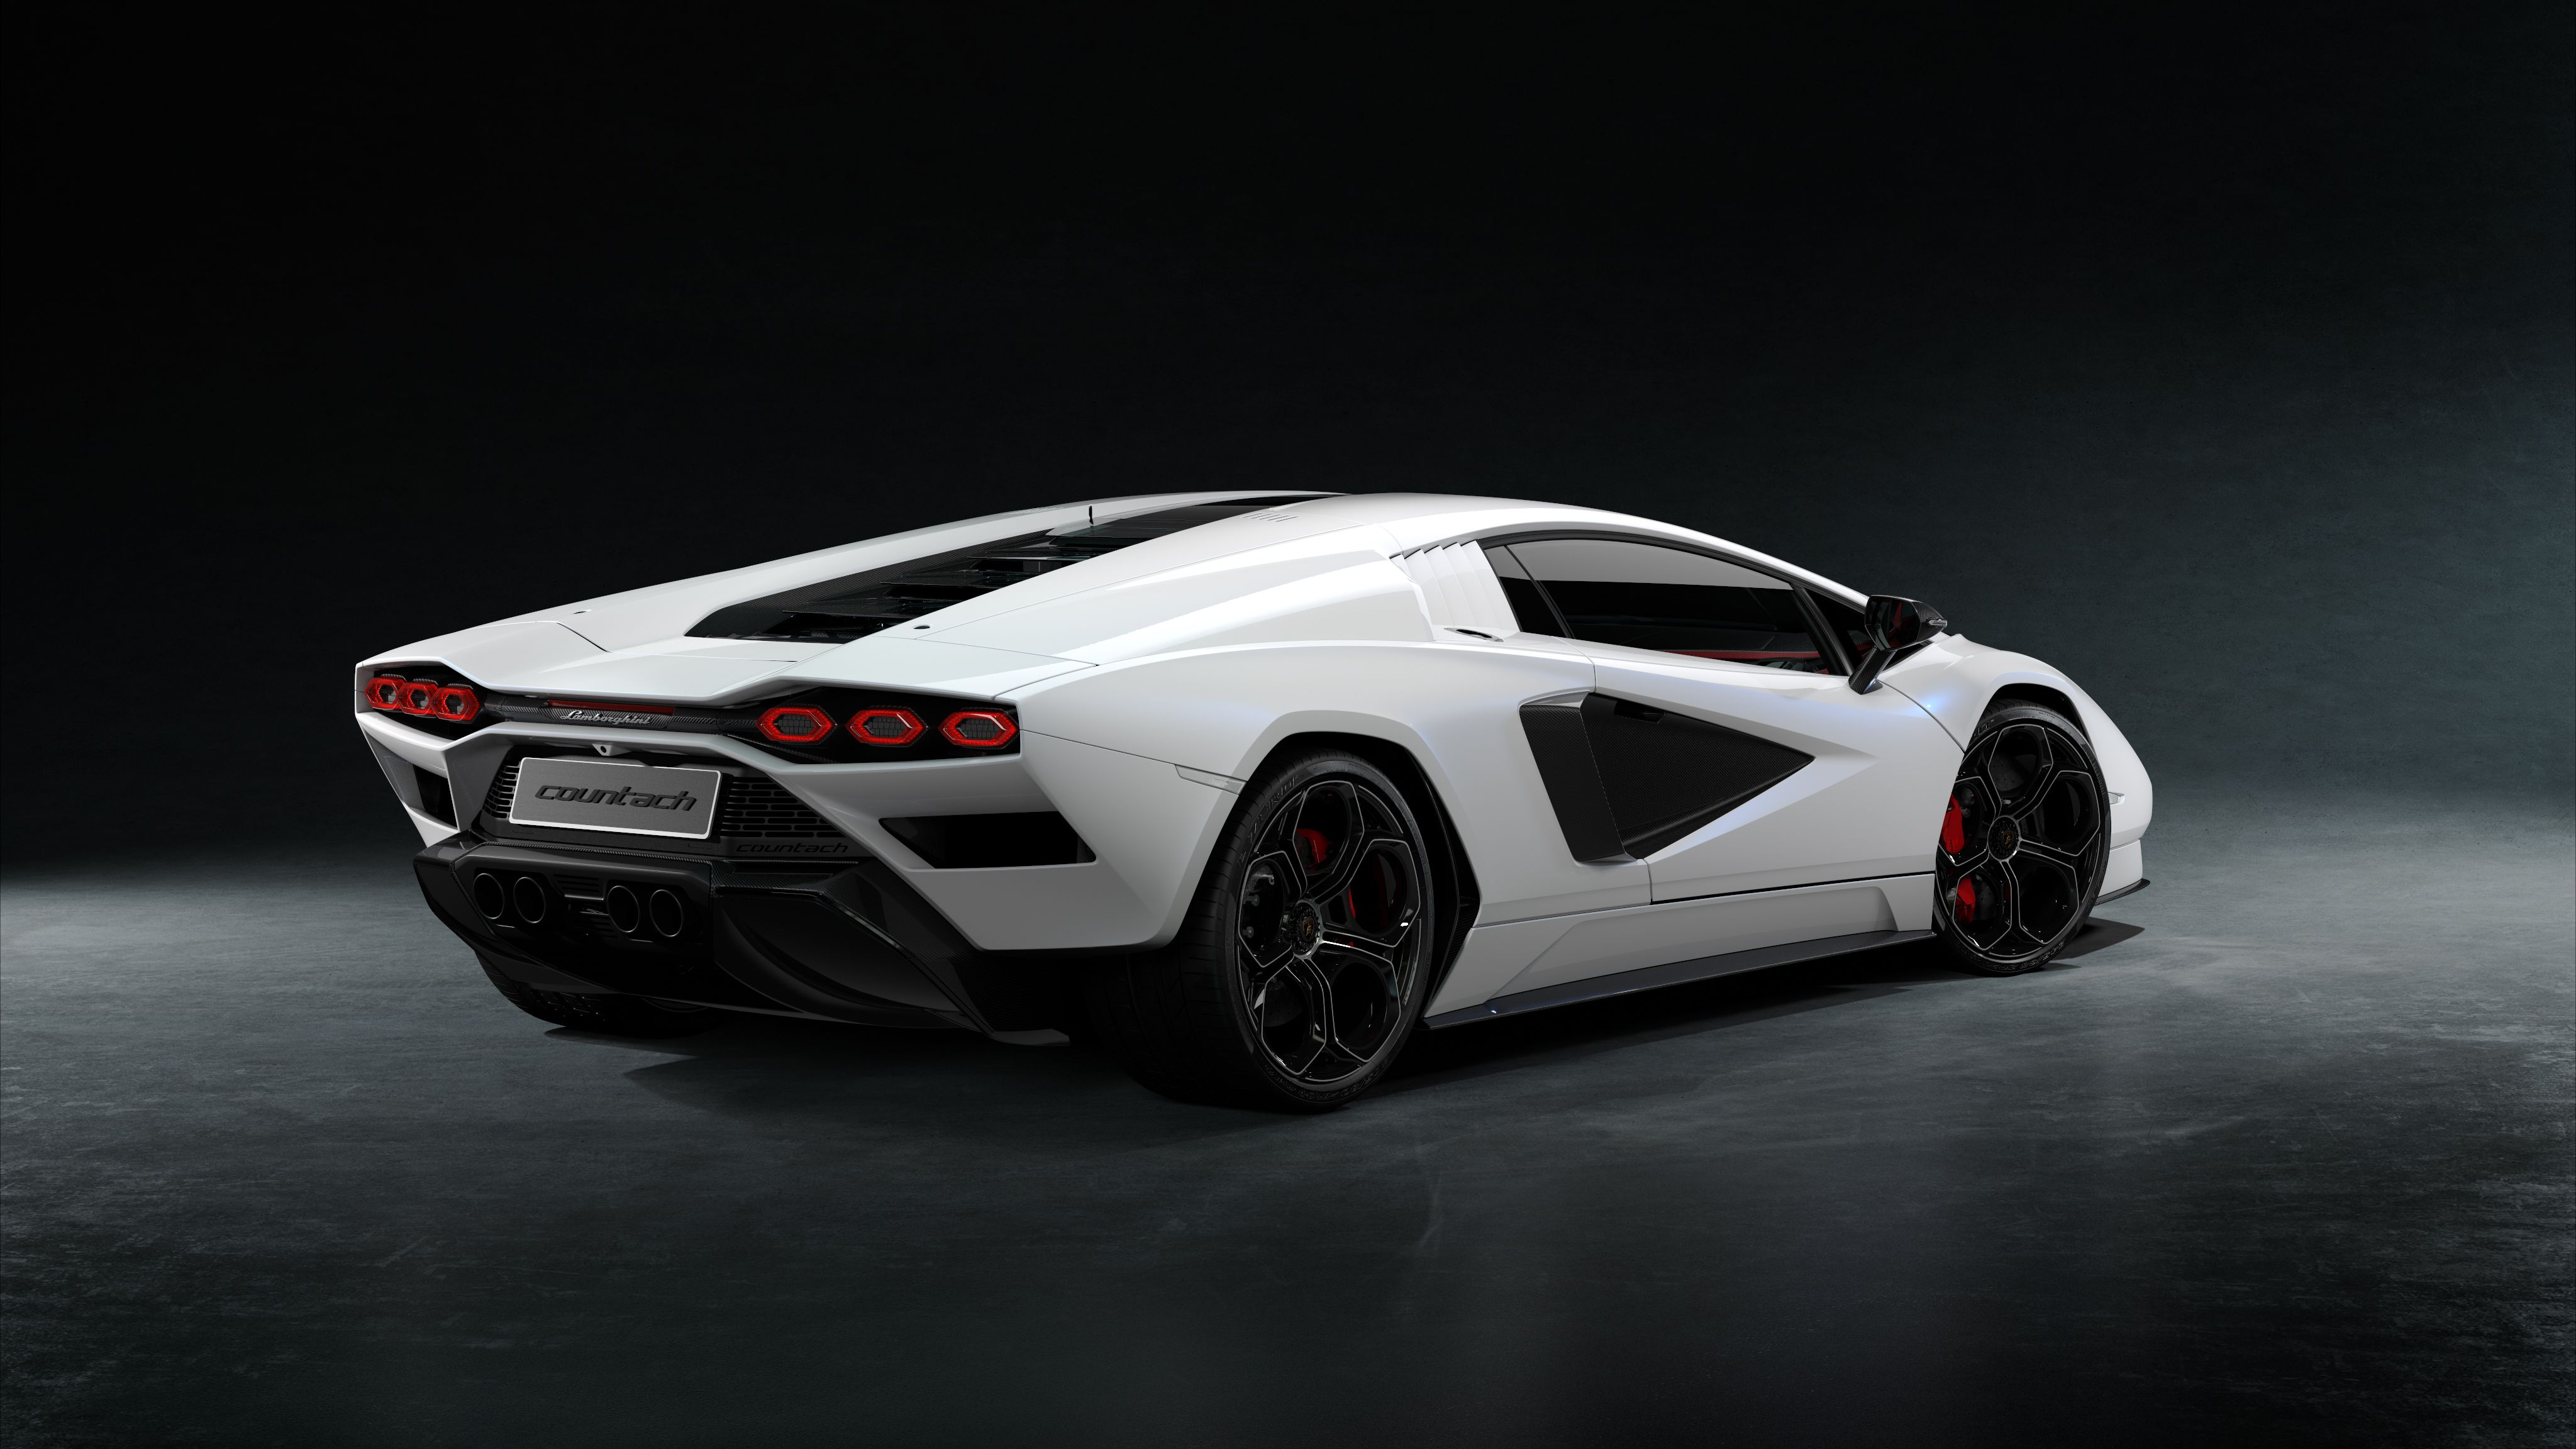
\includegraphics[width=\linewidth]{images/lambo.jpeg}
\end{center}

\vspace{1in}

\begin{center}
    Università di Bologna\\
    Campus di Cesena\\
    Facoltà di Ingegneria e Scienze Informatiche
\end{center}

\newpage

\mbox{}

\newpage

\tableofcontents

\newpage

\section{Analisi dei requisiti}
\subsection{Intervista}
La concessionaria desidera che vengano mantenuti in memoria i dati dei propri
clienti con nome, cognome, numero di telefono ed opzionalmente email. Per poter
acquistare una autovettura bisogna disporre del badge di iscrizione alla
concessionaria rinnovabile annualmente che identifica il cliente.\\
Oltre ai clienti iscritti alla concessionaria potrebbero venire in visita
persone comuni non iscritte delle quali non si ha interesse nel memorizzarle.
Considerando che non tutte le vetture in vendita sono presenti fisicamente nel
salone della concessionaria si richiede un sistema per la creazione di ordini
che possono includere più di una vettura. Ogni cliente possiede uno storico di
super car acquistate, utile alla azienda ai fini di marketing.\\
I dipendenti vengono distinti per nome, cognome, email aziendale e numero di
telefono aziendale e hanno uno storico delle proprie auto vendute. Inoltre, i
dipendenti, possono ottenere un bonus sullo stipendio se raggiungono un numero
minimo di vendite mensili, questo sistema incoraggia le vendite.\\
Le vetture del catalogo che andranno mantenute in memoria sono definite dal
codice di telaio, marca, modello, colore, unico segmento [Sport, Luxury,
SUV,...], cavalli potenza, prezzo, e colore. Inoltre variano in base al
restyling. Una vettura può essere acquistata da un solo cliente che ogni 2 anni
potrà portarla nel officina della concessionaria per manutenzione ordinaria,
servizio gratuito esplicitato al momento del ordine. Una autovettura può essere
prodotta da un solo produttore detto anche \textit{Casa Automobilista}, la quale
per lo stesso modello crea diversi restyling.\\
La super car può essere equipaggiata da optional differenti, i quali possono
essere prodotti da fornitori diversi. Ogni segmento possiede i propri optional
che alle volte vengono condivisi da più segmenti (ad esempio il Clima Automatico
o il Cambio Automatico sono optional presenti in ogni segmento a differenza del
Paraurti rinforzato che può essere montato solo su vetture di grandi dimensioni
presenti nei segmenti SUV ed OffRoad). Ogni optional è definito da una
descrizione, un codice prodotto e un livello di qualità di costruzione da 1 a
10.\\
Un cliente della concessionaria può eventualmente mettere in conto-vendita le
proprie autovetture ma solo nel caso rispettino gli standard qualitativi della
concessionaria, viene quindi fatta una valutazione da un professionista della
concessionaria che redige una scheda che descrive lo stato della vettura da
affiancare al contratto di conto-vendita. Il conto-vendita é composto da una
sola autovettura ed il prezzo è scelto dal proprietario. Nel contratto di
conto-vendita è presente una commissione che la concessionaria trattiene.

\subsection{Rilevamento delle ambiguità e analisi del intervista} 

Si procede con un analisi del testo frammentanta, analizzando parte per parte e
costruendo i relativi scheletri degli schemi E/R .

\subsubsection{Clienti}
\textbf{La concessionaria desidera che vengano mantenuti in memoria i dati dei
propri clienti con nome, cognome, numero di telefono ed opzionalmente email. Per
poter acquistare una autovettura bisogna disporre del badge di iscrizione alla
concessionaria rinnovabile annualmente che identifica il cliente.}

Si rileva che il cliente è un concetto fondamentale per la concessionaria e
viene identificato con un tesserino chiamato BADGE. Non è uno strumento
realmente utile alla concessionaria per la vendita, bensì è uno struemnto di
marketing che vuole fidelizzare il cliente trasmettendo un senso di esclusività.
Il BADGE è unico ed appartene ad un solo proprietario che a sua volta ne può
avere uno solo. Il BADGE, inoltre, è rinnovabile annualmente quindi mantiene lo
stesso codice ma cambia la data di scadenza.


\begin{center}
    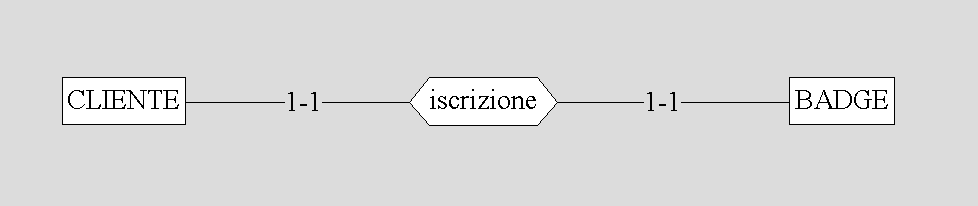
\includegraphics[width=\linewidth]{images/cliente.png}
\end{center}

\subsubsection{Ordini}
\textbf{Oltre ai clienti iscritti alla concessionaria potrebbero venire in
visita persone comuni non iscritte delle quali non si ha interesse nel
memorizzarle. Considerando che non tutte le vetture in vendita sono presenti
fisicamente nel salone della concessionaria si richiede un sistema per la
creazione di ordini che possono includere più di una vettura. Ogni cliente
possiede uno storico di super car acquistate, utile alla azienda ai fini di
marketing.}

Non c'é interesse nel memorizzare i dati di persone comuni in visita alla
concessionaria. Per quanto riguarda i clienti invece, si vuole mantenere uno
storico delle supercar acquistate e dare la possibilità di creare ordini che
possono includere più di una vettura. Viene quindi introdotta l'entità ORDINE
che rappresenta un contratto di acquisto. Lo storico delle supercar acquistate
da un cliente è utile alla concessionaria al fine di conoscere i gusti del
cliente e proporre nuovi modelli che gli potrebbero interessare.

\begin{center}
    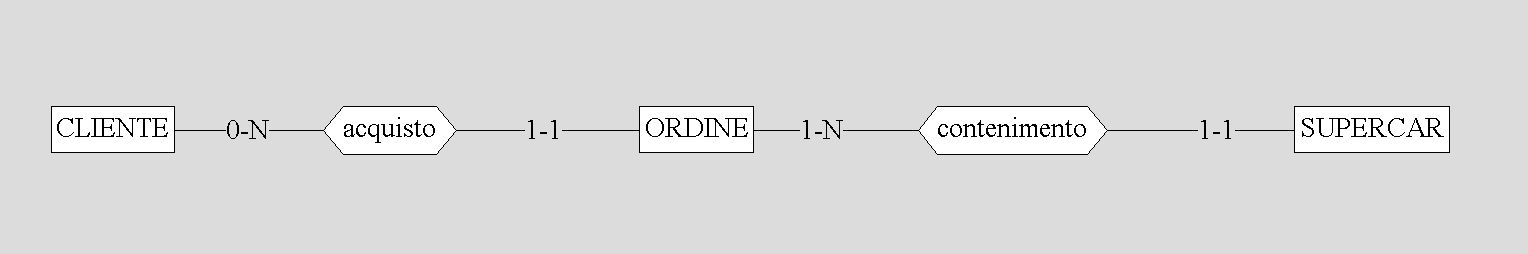
\includegraphics[width=\linewidth]{images/ordine.png}
\end{center}

\subsubsection{Dipendenti}
\textbf{I dipendenti vengono distinti per nome, cognome, email aziendale e
numero di telefono aziendale e hanno uno storico delle proprie auto vendute.
Inoltre, i dipendenti, possono ottenere un bonus sullo stipendio se raggiungono
un numero minimo di vendite mensili, questo sistema incoraggia le vendite.}

A seguito di ulteriori indagini si rileva che ad identificare i dipendenti è la
mail aziendale, la quale è utile anche nella fase di log in nel applicativo.
Inoltre, viene tenuta memoria delle supercar vendute dai dipendenti per
valutarne il lavoro e per assegnare un bonus (mensile) nel caso abbiano superato
un obbiettivo di supercar vendute. Viene quindi introdotta l'entià STIPENDIO per
la memorizzazione opzionale del bonus. Per memorizzare lo storio delle vendite
invece si sfrutta l'entità ORDINE.

\begin{center}
    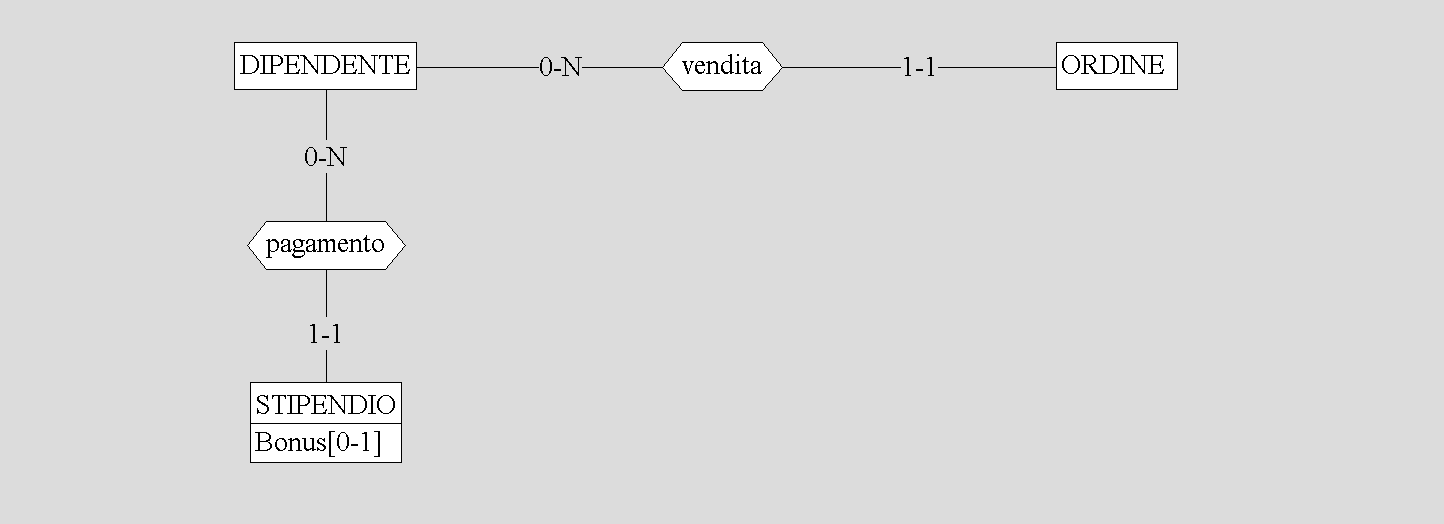
\includegraphics[width=\linewidth]{images/dipendente.png}
\end{center}

\subsubsection{Supercar}
\textbf{Le vetture del catalogo che andranno mantenute in memoria sono definite
dal codice di telaio, marca, modello, colore, unico segmento [Sport, Luxury,
SUV,...], cavalli potenza, prezzo, e colore. Inoltre variano in base al
restyling. Una vettura può essere acquistata da un solo cliente che ogni 2 anni
potrà portarla nel officina della concessionaria per manutenzione ordinaria,
servizio gratuito esplicitato al momento del ordine. Una autovettura può essere
prodotta da un solo produttore detto anche \textit{Casa Automobilista}, la quale
per lo stesso modello crea diversi restyling.}

Il codice del telaio è l'identificatore fondamentale di una qualsiasi vettura.
Il cliente, unico proprietario di una certa vettura acquistata, può portarla in
revisione dal officina della concessionaria ogni 2 anni gratuitamente.\\
Si pone particoalre attenzione sul restylng di una supercar in quanto per un
certo modello possono essere prodotte diverse versioni. Viene quindi introdotta
l'entità VERSIONE che separa alcuni attributi dalla entità SUPERCAR. Il prezzo
ed il colore ad esempio variano in base alla versione della vettura quindi vanno
a caratterizzare una VERSIONE e non il modello; il primo per via delle leggi di
mercato, il secondo a causa di vetture a tiratura limitana che vengono prodotte
con colori particoalri. Inoltre l'entità VERSIONE definisce anche istanze di
vetture che non hanno ricevuto un nuovo aggiornamento in quanto in termini
assoluti si trovano alla loro prima versione, ne segue che non esiste una
SUPERCAR senza almeno una VERSIONE. Per quanto riguarda il modello (sinominimo
di SUPERCAR), esso è prodotto da una CASA AUTOMOBILISTICA che attraverso il
proprio nome definisce la marca di una certa SUPERCAR.

\begin{center}
    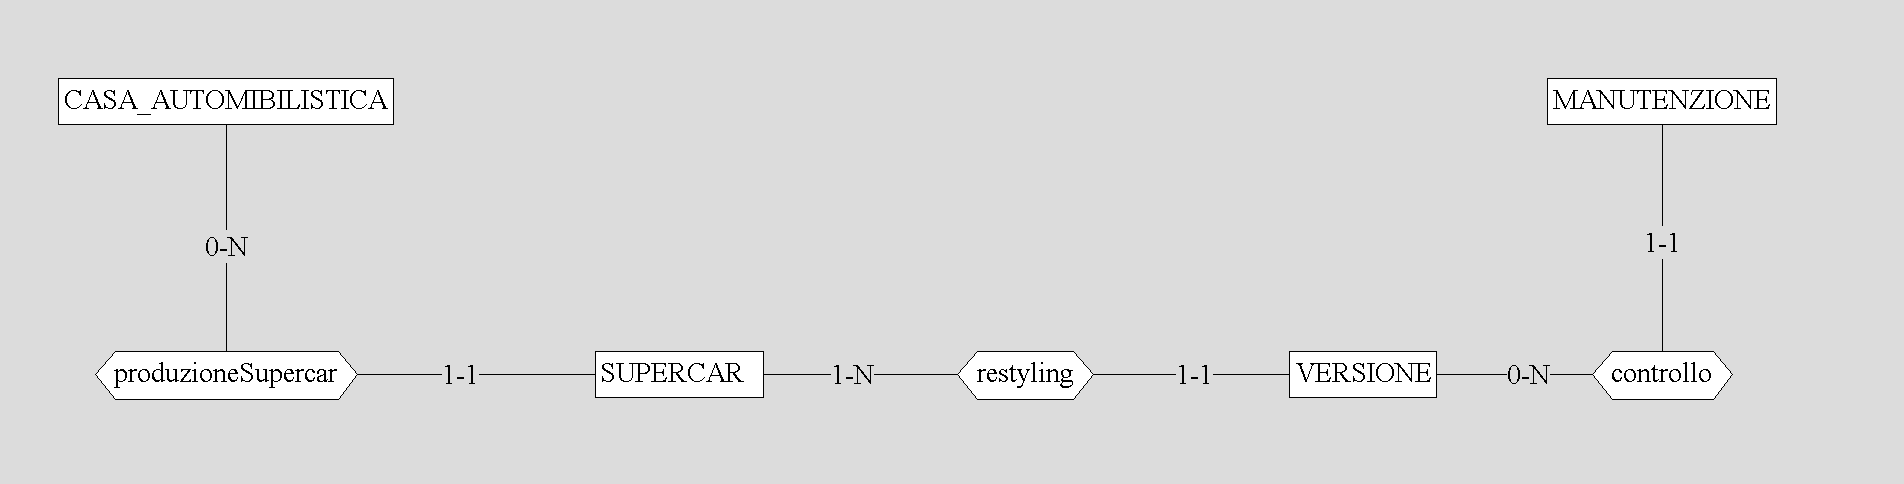
\includegraphics[width=\linewidth]{images/versione.png}
\end{center}

\subsubsection{Optional e Produttore}
\textbf{La super car può essere equipaggiata da optional differenti, i quali
possono essere prodotti da fornitori diversi. Ogni segmento possiede i propri
optional che alle volte vengono condivisi da più segmenti (ad esempio il Clima
Automatico o il Cambio Automatico sono optional presenti in ogni segmento a
differenza del Paraurti rinforzato che può essere montato solo su vetture di
grandi dimensioni presenti nei segmenti SUV ed OffRoad). Ogni optional è
definito da una descrizione, un codice prodotto e un livello di qualità di
costruzione da 1 a 10.}

Si decide di trattare i segmenti come entità identificate dal proprio nome e
seguite da una descrizione. In generale un SEGMENTO è nient altro che il termine
tecnico per definire la categoria. Una supercar può equipaggiare optional
differenti, i quali devono appartenere allo stesso segmento della vettura. Gli
optional possono essere prodotti da diversi produttori, i quali pssono anche
essere CASE AUTOMOBILISTICHE. Si introduce quindi una gerarchia Totale e
Sovrapposta che definisce i produttori di optional e le case automobilistiche.

\begin{center}
    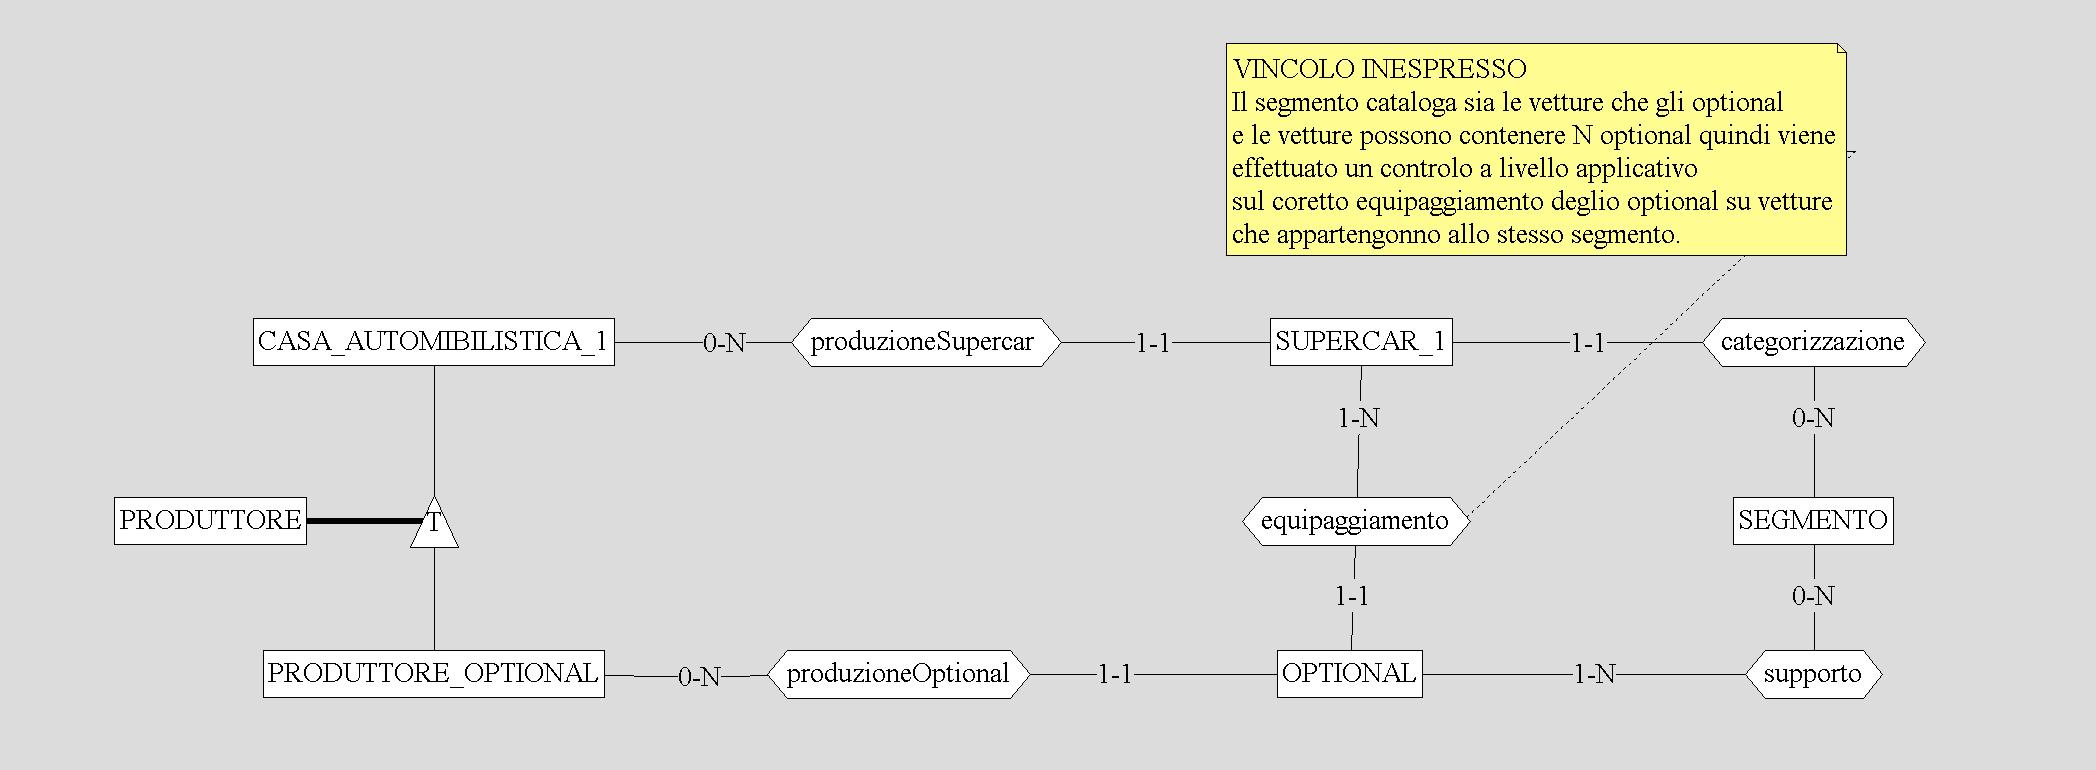
\includegraphics[width=\linewidth]{images/optional.png}
\end{center}

\subsubsection{Conto-Vendita}
\textbf{Un cliente della concessionaria può eventualmente mettere in
\hyphenation{conto-vendita} le proprie autovetture ma solo nel caso rispettino
gli standard qualitativi della concessionaria, viene quindi fatta una
valutazione da un professionista della concessionaria che redige una scheda che
descrive lo stato della vettura da affiancare al contratto di
\hyphenation{conto-vendita}. Il \hyphenation{conto-vendita} é composto da una
sola autovettura ed il prezzo è scelto dal proprietario.\\ 
Nel contratto di \hyphenation{conto-vendita} è presente una commissione che la
concessionaria trattiene.}

Si rileva che il conto-vendita è un contratto di vendita che viene stipulato tra
concessionaria e CLIENTE. A seguito di ulteriori indagini si rileva che la
vettura in conto-vendita deve essere inserita nella struttura dati proprio come
una SUPERCAR comunemente venduta dalla concessionaria. Viene introdotta l'entità
CONTO-VENDITA che rappresenta il contratto alla quale viene affiancata la SCHEDA
DI VALUTAZIONE. E' importante precisare che non c’è un dipendente in particolare
ad occuparsi della conto-vendita ed è obbiettivo di tutti i dipendenti la più
rapida conclusione di questi contratti. In questo modo la vendita relativa ad
una vettura in conto-vendita non aumenta il numero di autovetture vendute dal
dipendente utili ad ottenere il bonus.

\begin{center}
    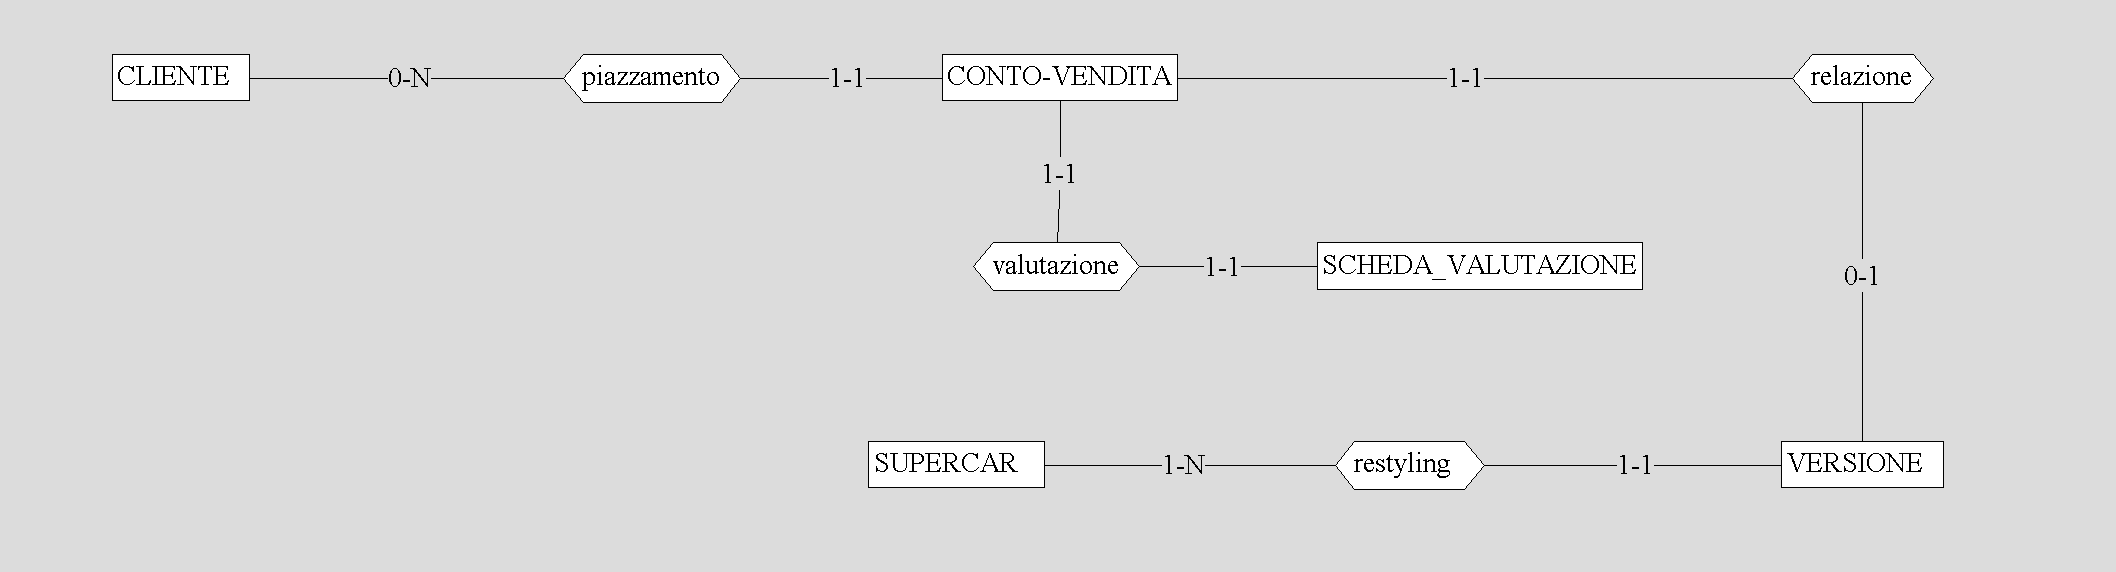
\includegraphics[width=\linewidth]{images/contovendita.png}
\end{center}

\newpage

\sloppy{\subsection{Definizione delle specifiche in linguaggio naturale
ed estrazione dei concetti principali}}

\begin{itemize}
    \item \textbf{CLIENTE}: compratore iscritto alla concessionaria
    \item \textbf{BADGE}: tesserino utile al riconoscimento dei clienti
    \item \textbf{DIPENDENTE}: venditore
    \item \textbf{ORDINE}: contratto di acquisto di una o più vetture
    \item \textbf{STIPENDIO}: paga mensile di un dipendente
    \item \textbf{CONTO-VENDITA}: contratto di vendita di una vettura per conto
    di un cliente
    \item \textbf{SCHEDA VALUTAZIONE}: descrive lo stato di una vettura in
    CONTO-VENDITA
    \item \textbf{VERSIONE}: nuova versione di una supercar basata sullo stesso
    modello\\ (es. Modello: Alfa Romeo Giulia, Versione: Edizione Anniversario)
    \item \textbf{SUPERCAR}: modello prodotto da una Casa Automobilistica. Alle
    volte chiamata anche comunaente \textit{Modello} oppure \textit{Vettura}.
    \item \textbf{MANUTENZIONE}: revisione di una super car (es. cambio del
    olio)
    \item \textbf{SEGMENTO}: genere/tipologia/categoria di supercar \\
    (es. Sport, SUV, Berlina, OffRoad,..)
    \item \textbf{OPTIONAL}: dispositivo che una vettura può equipaggiare
    opzionalmente    
    \item \textbf{CASA AUTOMOBILISTICA}: azienda produttrice di autovetture
    \item \textbf{PRODUTTORE OPTIONAL}: azienda produttrice di optional
\end{itemize}

\section{Progettazione Concettuale}

\subsection{Schema scheletro assemblato}

\begin{center}
    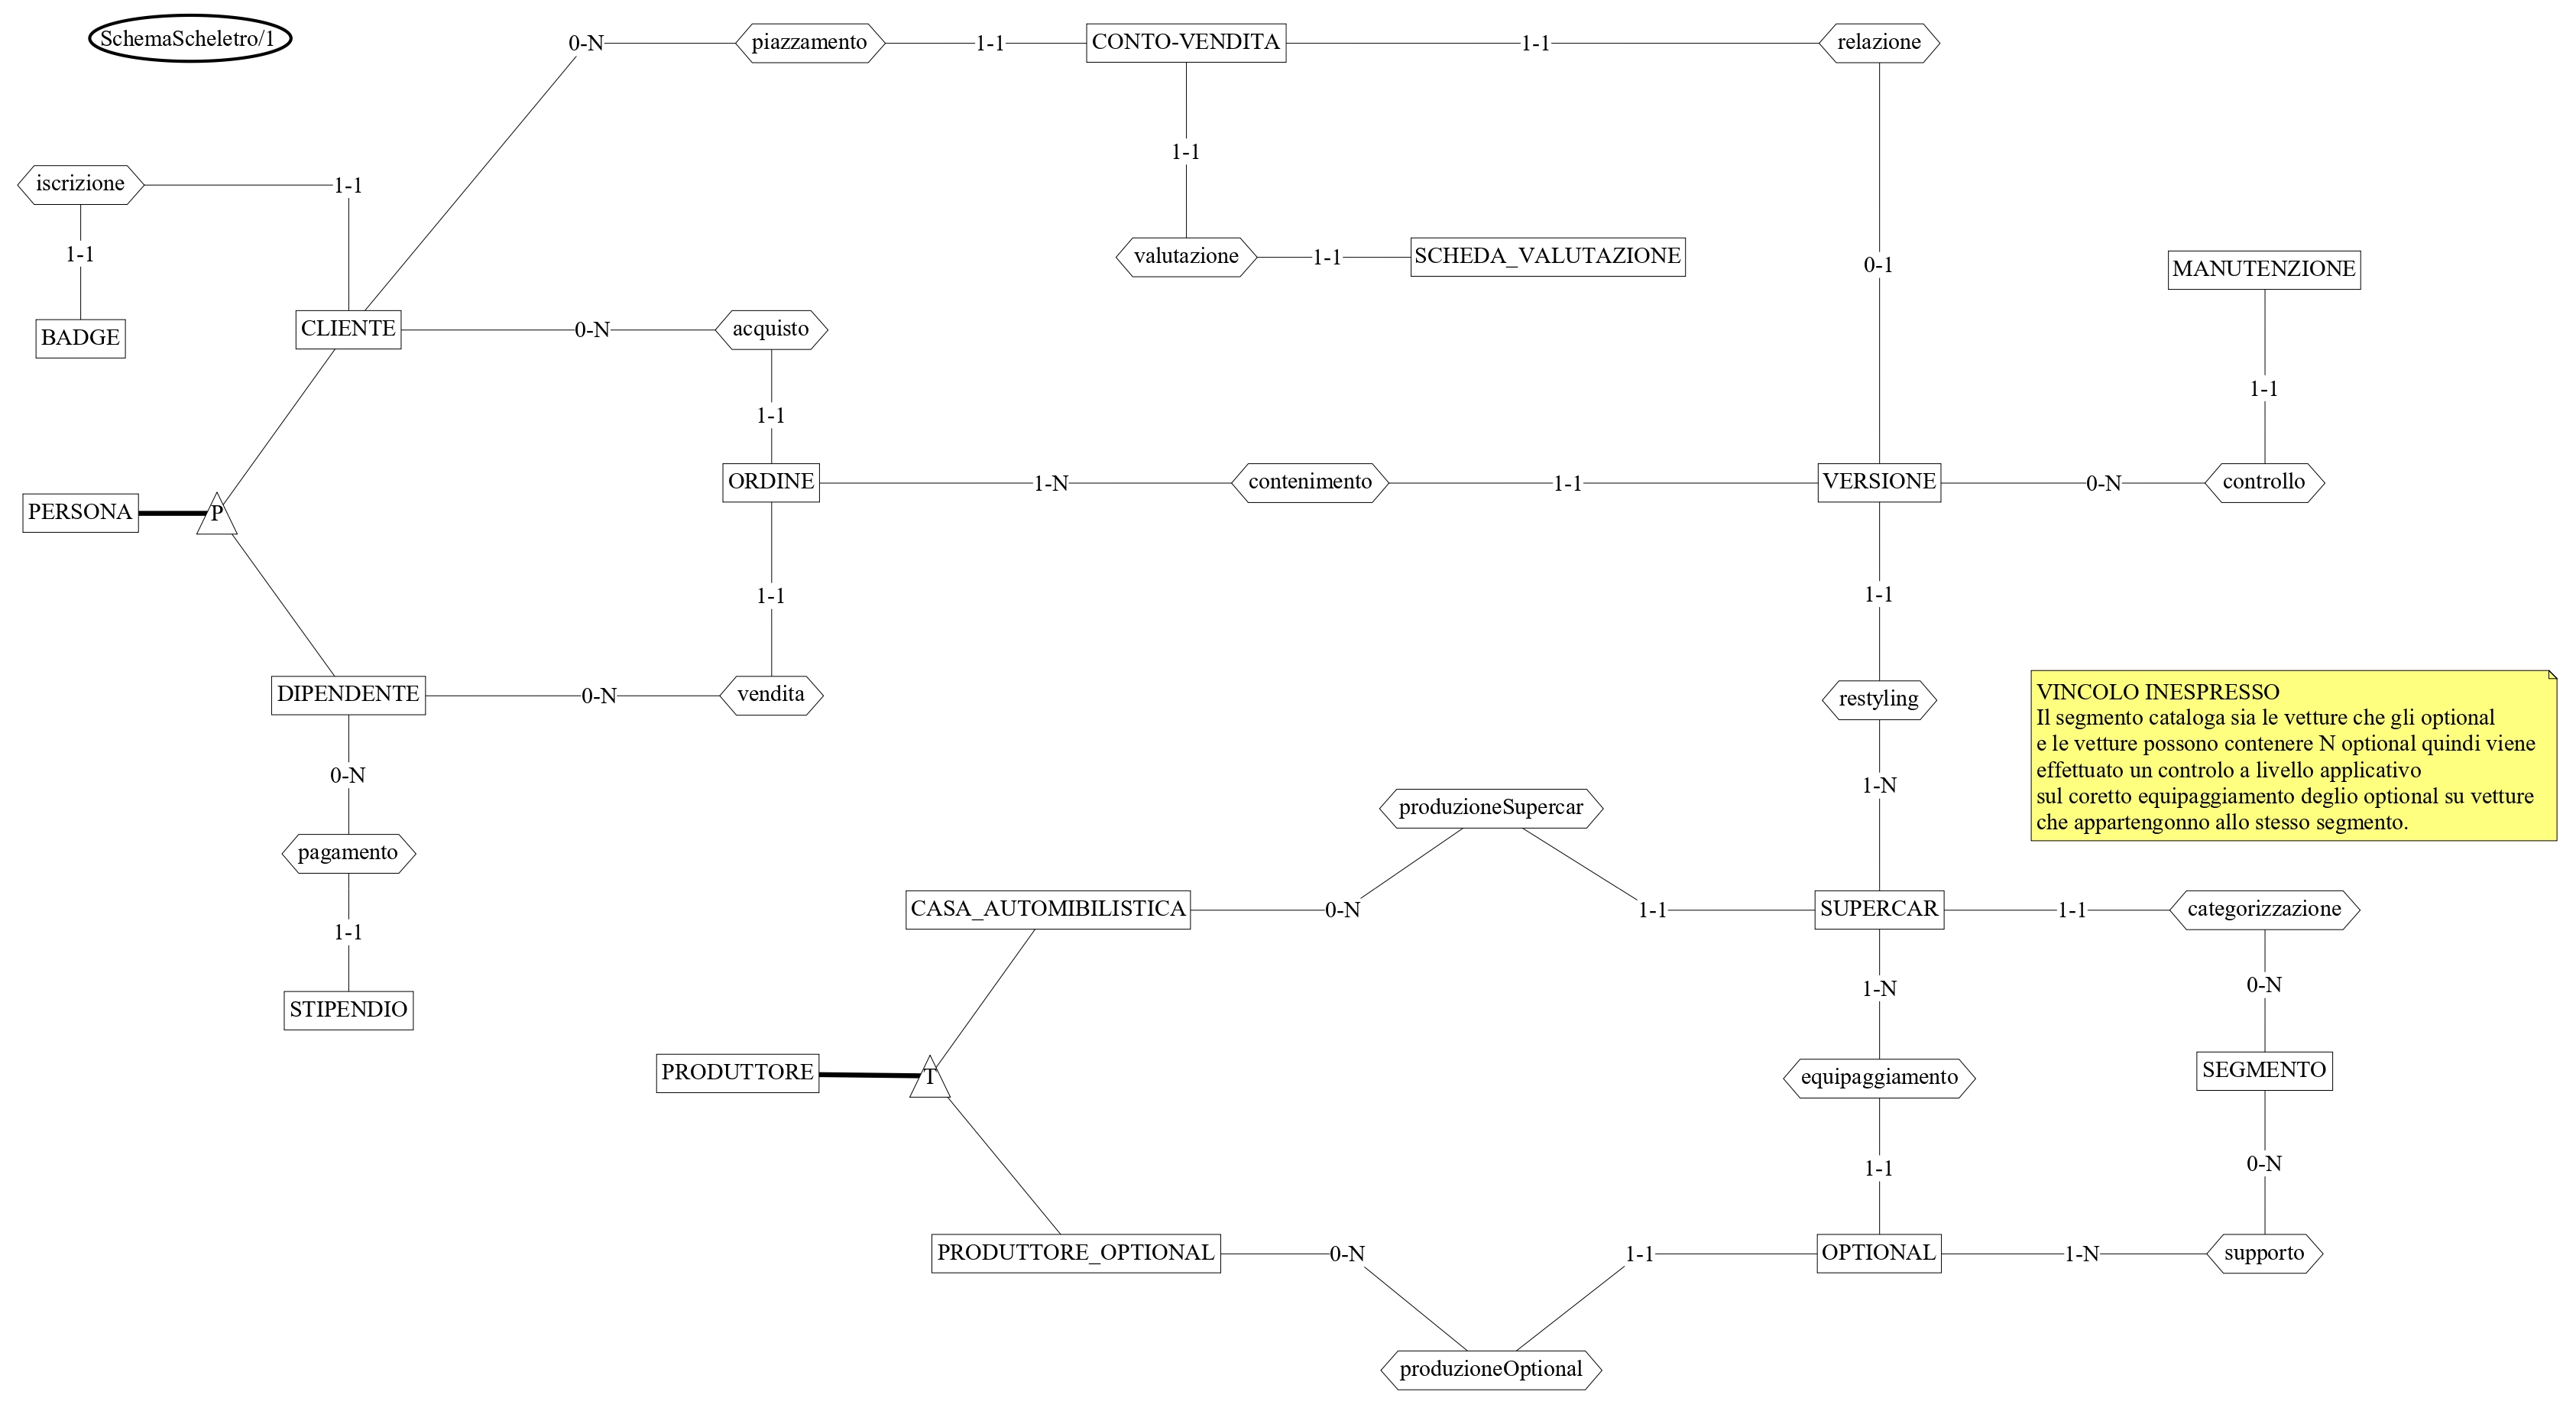
\includegraphics[scale=0.75, angle=90]{images/schemaScheletro.png}
\end{center}

\newpage

\subsection{Schema concettuale finale}
\begin{center}
    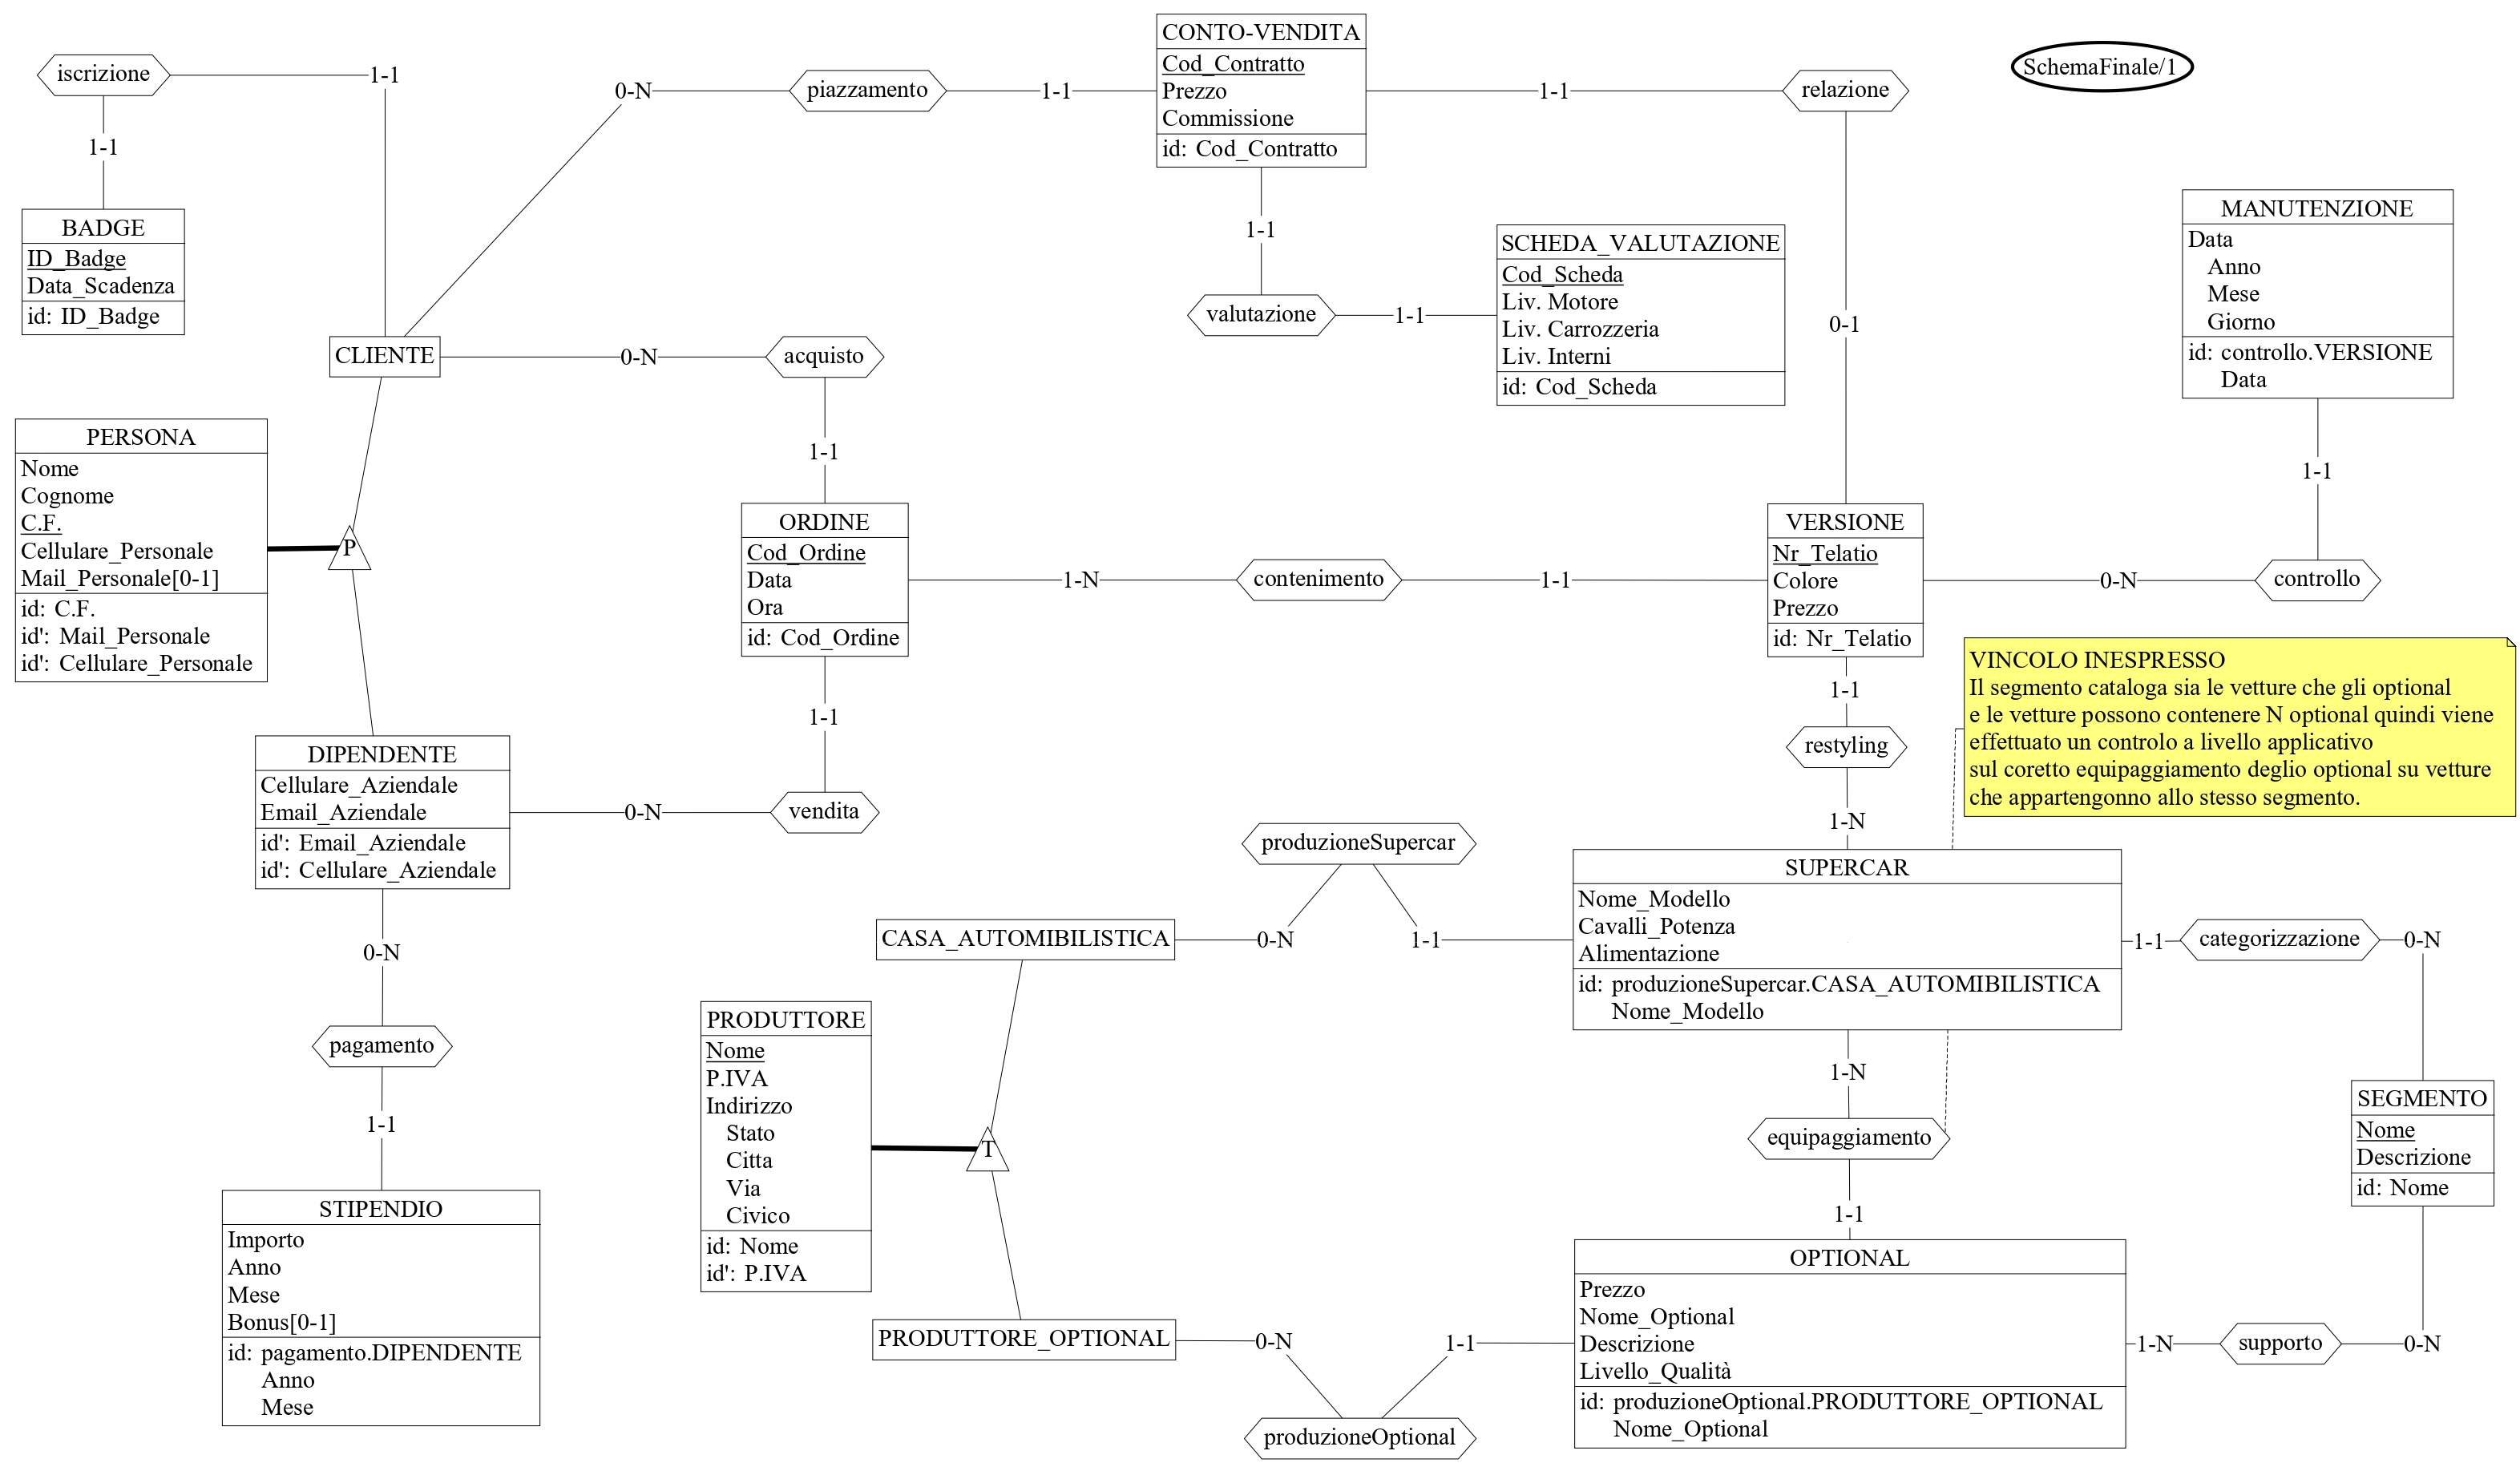
\includegraphics[scale=0.85, angle=90]{images/schemaFinale.png}
\end{center}

\newpage

\section{Progettazione Logica}

\subsection{Stima del volume dei dati}

La seguente stima di dati viene valutata ad un anno dalla apertura della
concessionaria nel mercato di una città di grande dimensioni (es. Milano). 

\begin{table}[htbp]
    \centering
    \small
    \rowcolors{2}{red!5!}{white}
    \begin{tabularx}{\textwidth}{c l c X }
        \rowcolor{red!20!}
        \textbf{Tipo} & \textbf{Concetto} & \textbf{Volume} & \textbf{Nota}\\
        E & CLIENTE & 400 & \\
        E & DIPENDENTE & 30 & \\
        E & ORDINE & 800 & Si stimano mediamente 2 ordine a cliente. \\
        E & BADGE & 400 & \\
        E & STIPENDIO & 390 & Mediamente ci sono 13 stipendi per dipendente. \\
        E & CONTO-VENDITA & 20 & \\
        E & SCHEDA VALUTAZIONE & 20 & \\
        E & VERSIONE & 1200 & In media in un ordine troviamo 1 oppure 2 vetture.
        \\
        E & MANUTENZIONE & 10 & Manutenzioni straordinarie dovute a difetti
                                lievi dovuti al trasporto. Le manutenzione
                                ordinarie non avevano modo di presentarsi ad un
                                anno dal apertura della concessioanria. \\
        E & SUPERCAR & 900 & Questo valore non è riferito solo alle supercar
                                rilasciate dalle case produttrici nel ultimo
                                anno ma anche di vetture di anni passati che a
                                loro volta hanno diverse versioni. \\
        
        E & SEGMENTO & 7 & Coupè, Hypercar, Berlina di Lusso, Berlina compatta,
        SUV, OffRoad, Sportiva \\
        R & Supporto & 1250 & Mediamente per ogni segmento ci sono un numero
                                considerevole di optional ma trattandosi di
                                vetture particolarmente lussuose il numero si
                                riduce in favore della qualità. \\
        E & OPTIONAL & 10'000 & \\
        E & CASA AUTOMOBILISTICA & 100 & \\
        E & PRODUTTORE OPTIONAL & 300 & \\  
        
    \end{tabularx}
    \label{tab:volume_table}
\end{table}


\subsection{Descrizione delle operazioni principali e stima della loro frequenza}

Le seguenti operazioni vanno a descrivere il comportamento di un dipendente tipo
(ad eccezione delle numero 6 e 9) della concessionaria. In parte sono operazioni
comuni di vendita, altre di rilevazione statistica al fine di analizzare il
mercato e preformare al meglio nelle vendite. 

\begin{table}[htbp]
    \centering
    \small
    \rowcolors{2}{red!5!}{white}
    \begin{tabularx}{\linewidth}{c X c}
      \rowcolor{red!20!}
      \textbf{Codice} & \textbf{Operazione} & \textbf{Frequenza} \\
      1 & Log In di un dipendente & 900 al mese \\
      2 & Inserimento di un nuovo cliente & 33 al mese \\
      3 & Visualizza le vetture acquistate da un cliente in un certo periodo in
      ordine crescente di data & 14 al mese \\
      4 & Visualizza gli optional di una certa azienda & 20 al mese \\
      5 & Inserimento di un nuovo ordine & 66 al mese \\
      6 & Aggiungere un contratto di conto vendita & 1.6 al mese \\
      7 & Visualizza i dipendenti che in un certo mese hanno ottenuto il bonus & 12
      al anno \\
      8 & Visualizza Top 10 supercar più vendute di un segmento & 3 al mese \\
      9 & Inserisci una nuova versione di una supercar & 75 al mese \\
      10 & Aggiungi manutenzione ad un veicolo & 500 all' anno \\
      11 & Visualizza i 5 clienti iscritti da più tempo &  20 all' anno \\
      12 & Visualizza le vetture che hanno eseguito manutenzione ordinaria in un
      certo anno & 5 all'anno \\
    \end{tabularx}
    \label{tab:tabella_frequenze}
\end{table}
\subsection{Schemi di navigazione e tabelle degli accessi}

Di seguito si riportano le tabelle degli accessi delle operazioni sopracitate.
Si considera il peso dello scritture doppio rispetto a quello delle letture.

\subsection{Log In di un dipendente}

\begin{table}[H]
    \centering
    \rowcolors{2}{red!5!}{white}
    \begin{tabular}{ c c c c }
        \rowcolor{red!20!}
        \textbf{Concetto} & \textbf{Costrutto} & \textbf{Accessi} &
        \textbf{Tipo}\\
        DIPENDENTE & E & 30 & L \\
    \end{tabular}\\
    \( 30L \rightarrow 900 \) al mese = \( 30L \times 900 =  27000\) al mese
\end{table}


\subsubsection{Inserimento di un nuovo cliente}

\begin{table}[H]
    \centering
    \rowcolors{2}{red!5!}{white}
    \begin{tabular}{ c c c c }
        \rowcolor{red!20!}
        \textbf{Concetto} & \textbf{Costrutto} & \textbf{Accessi} &
        \textbf{Tipo}\\
        CLIENTE & E & 1 & S \\
        BADGE & E & 1 & S \\
    \end{tabular}\\
    \( 2S \rightarrow 33 \) al mese = \( 2S \times 2 \times 33 = 132 \) al mese
\end{table}

\subsubsection{Visualizza le vetture acquistate da un cliente in un certo periodo in
ordine crescente di data}

Accedendo alla sezione di un cliente attraverso il suo badge analizziamo i suoi
ordini, i quali mediamente contengono una supercar, successivamente eseguiamo
una lettura anche sul modello per avere le informazioni complete.

\begin{center}
    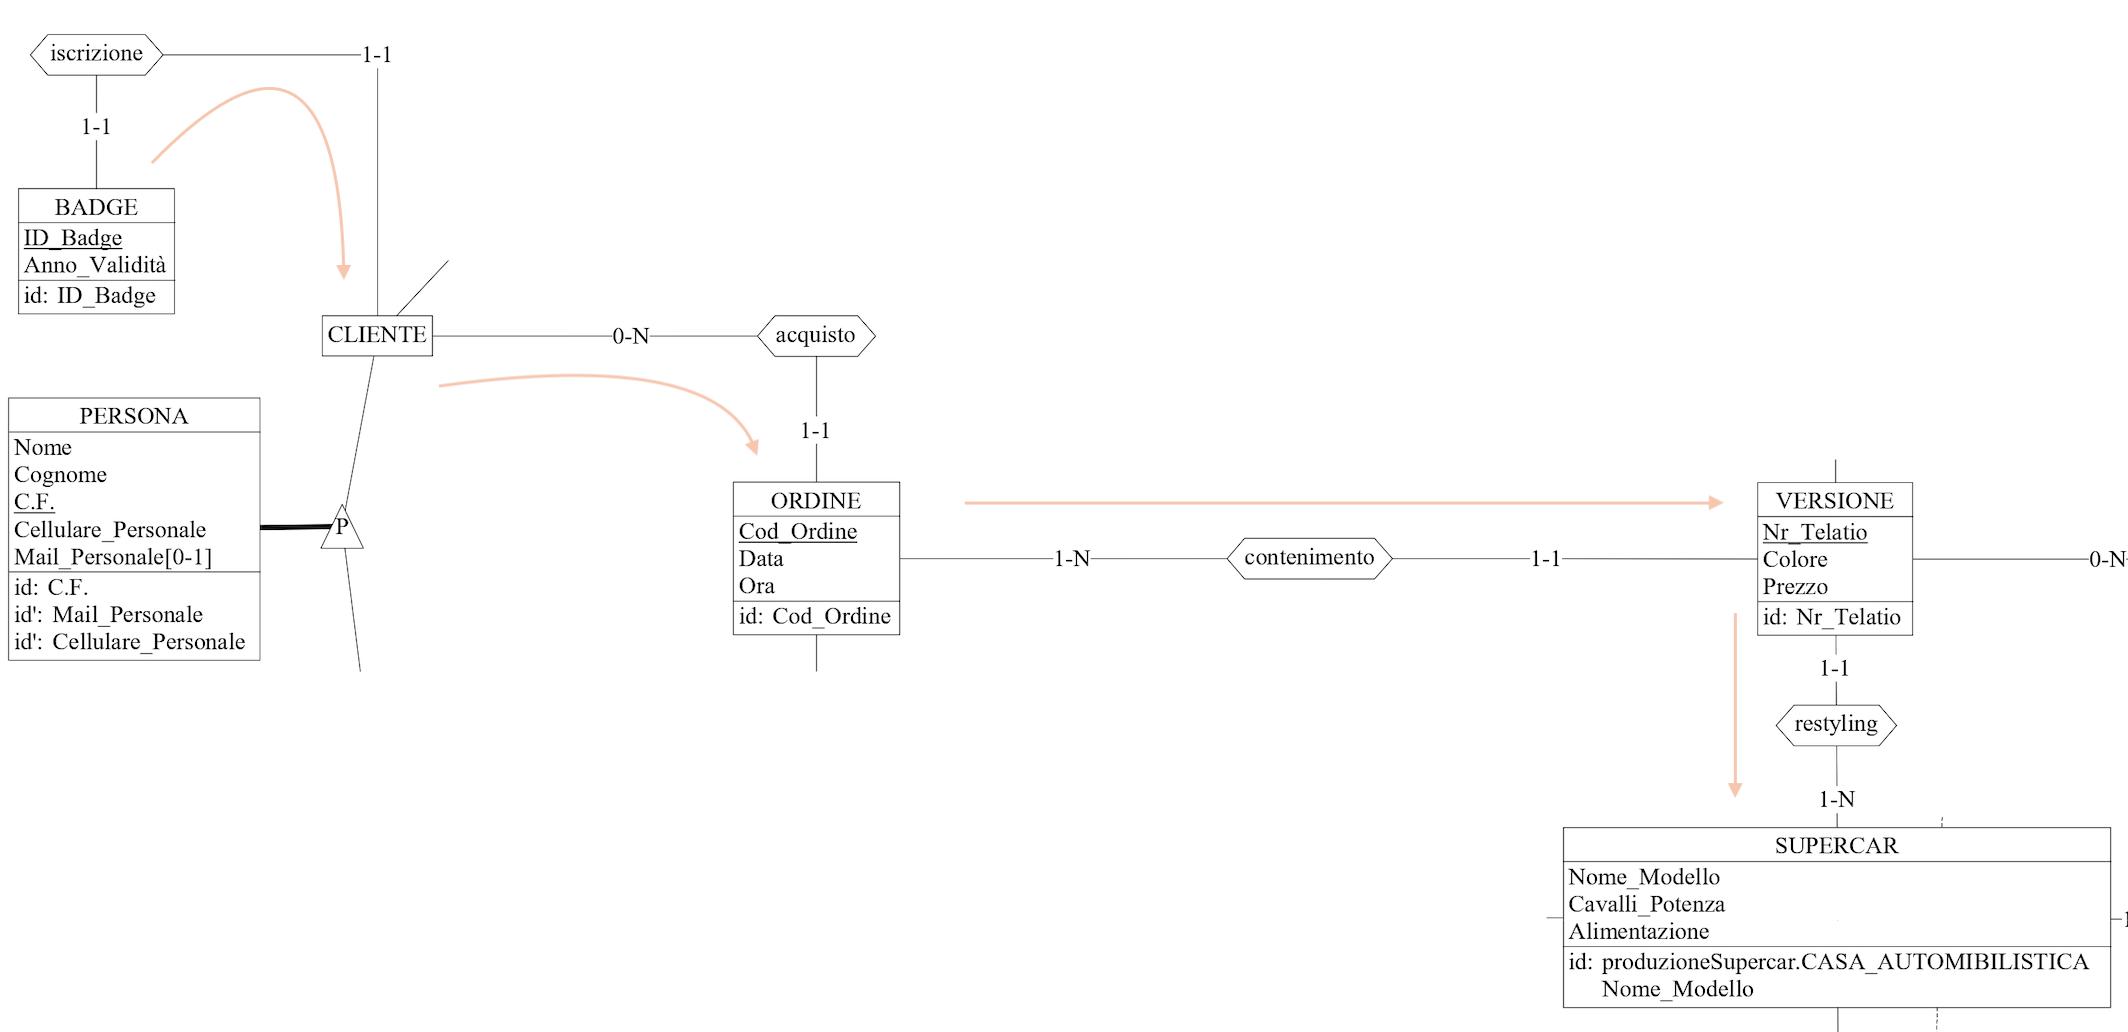
\includegraphics[scale=0.40]{images/acquistiCliente.png}
\end{center}

\begin{table}[H]
    \centering
    \rowcolors{2}{red!5!}{white}
    \begin{tabular}{ c c c c }
        \rowcolor{red!20!}
        \textbf{Concetto} & \textbf{Costrutto}  & \textbf{Accessi} &
        \textbf{Tipo}\\ 
        BADGE & E & 1 & L \\ 
        CLIENTE & E & 1 & L \\ 
        ORDINE & E & 2 & L \\ 
        VERSIONE & E & 3 & L \\ 
        SUPERCAR & E & 3 & L \ \end{tabular}\\
        \( 10L  \rightarrow 14 \) al mese = \( 10 \times 14 = 140 \) al mese
\end{table}

\subsubsection{Visualizza gli optional di una certa azienda} \label{Visualizza
gli optional di una certa azienda}

Data una certa azienda vado a leggere tutti gli optional che produce. Mediamente
saranno 10'000 Optional / 300 Aziende produttrici di optional = 33 .

\begin{center}
    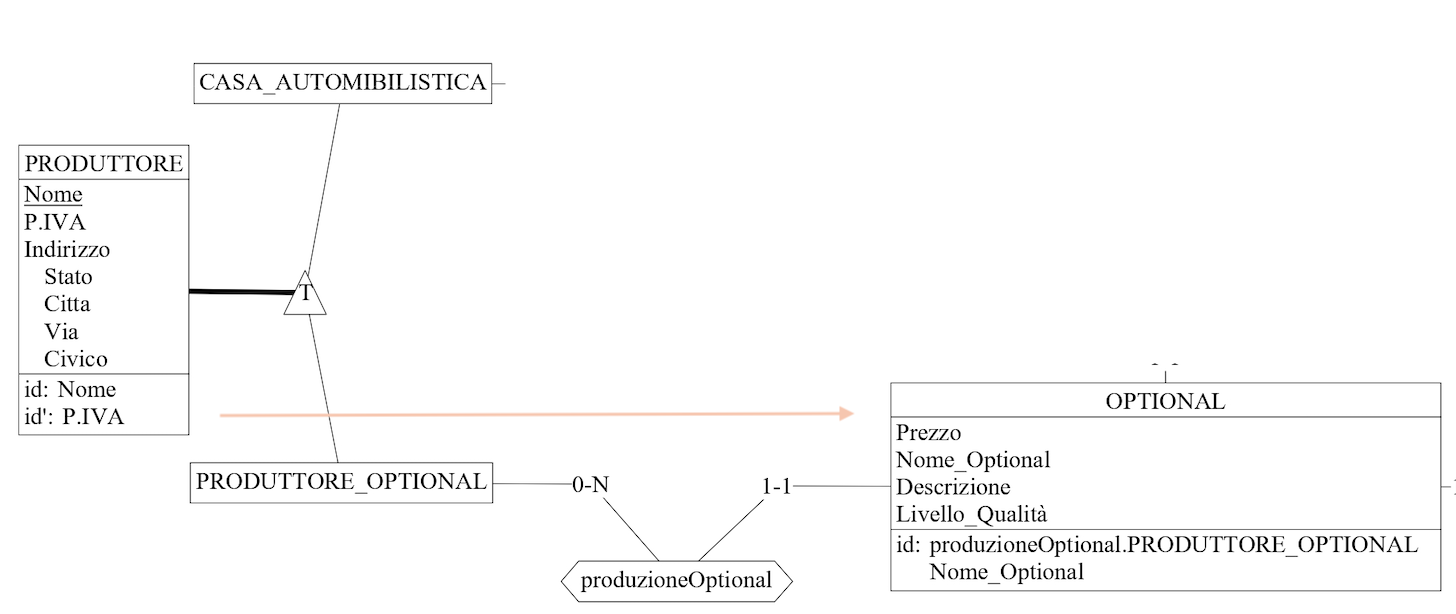
\includegraphics[scale=0.50]{images/optionalProduttore.png}
\end{center}

\begin{table}[H]
    \centering
    \rowcolors{2}{red!5!}{white}
    \begin{tabular}{ c c c c } 
        \rowcolor{red!20!}
        \textbf{Concetto} & \textbf{Costrutto} & \textbf{Accessi} &
        \textbf{Tipo}\\ 
        PRODUTTORE OPTIONAL & E & 1 & L \\ 
        OPTIONAL & E & 33 & L \\ 
    \end{tabular}\\
    \( 34L \rightarrow 20\) al mese = \( 34 \times 20 = 680 \) al mese
\end{table}

\subsubsection{Inserimento di un nuovo ordine} \label{Inserimento di un nuovo
ordine}

\begin{table}[H]
    \centering
    \rowcolors{2}{red!5!}{white}
    \begin{tabular}{ c c c c } 
        \rowcolor{red!20!}
        \textbf{Concetto} & \textbf{Costrutto} & \textbf{Accessi} &
        \textbf{Tipo}\\ 
        ORDINE & E & 1 & S \\ 
        CLIENTE & E & 1 & L \\ 
        DIPENDETE & E & 1 & L \\ 
        VERSIONE & E & 2 & L \\
        SUPERCAR & E & 2 & L \\ 
    \end{tabular}\\
    \( 1S + 6L \rightarrow \) 66 al mese = \( 1S \times 2 \times 66 + 6L \times
    66 = 506 \) al mese
\end{table}

\subsubsection{Aggiungere un contratto di conto vendita} \label{Aggiungere un
contratto di conto vendita}

\begin{table}[H]
    \centering
    \rowcolors{2}{red!5!}{white}
    \begin{tabular}{ c c c c } 
        \rowcolor{red!20!}
        \textbf{Concetto} & \textbf{Costrutto} & \textbf{Accessi} &
        \textbf{Tipo}\\ 
        CONTO VENDITA & E & 1 & S \\ 
        SCHEDA VALUTAZIONE & E & 1 & S \\ 
        CLIENTE & E & 1 & L \\ 
        VERSIONE & E & 1 & S \\ 
        SUPERCAR & E & 1 & S \\ 
    \end{tabular}\\
    \(4S + 1L \rightarrow \) 1.6 al mese = \( 4S \times 2 \times 1.6 + 1L \times
    1.6 = 14.4 \) al mese  
\end{table}

\subsubsection{Visualizza i dipendenti che in un certo mese hanno ottenuto il
bonus} 

\begin{center}
    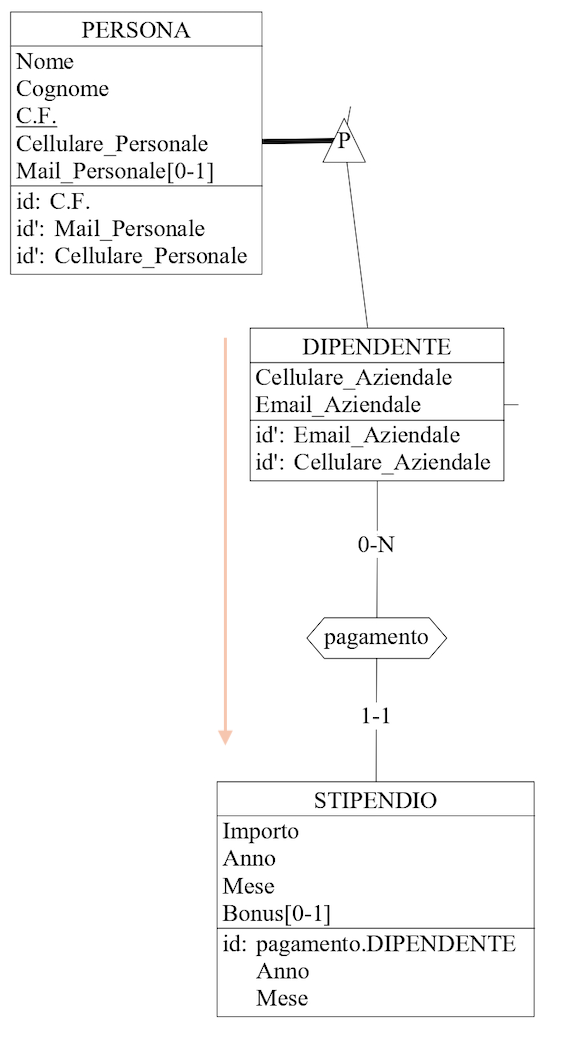
\includegraphics[scale=0.50]{images/bonusDipendenti.png}
\end{center}

\begin{table}[H]
    \centering
    \rowcolors{2}{red!5!}{white}
    \begin{tabular}{ c c c c } 
        \rowcolor{red!20!}
        \textbf{Concetto} & \textbf{Costrutto} & \textbf{Accessi} &
        \textbf{Tipo}\\ 
        DIPENDENTE & E & 30 & L \\ 
        STIPENDIO & E & 30 & L \\ 
    \end{tabular}\\
    \( 60L \rightarrow 12 \) all'anno = \( 60L \times 12 = 720 \) all'anno
\end{table}

\subsubsection{Visualizza Top 10 supercar più veloci di un segmento}

Dato un certo segmento vado a ordinare le supercar appartenenti prendendo come
parametro i Cavalli Potenza. In media abbiamo 900 supercar / 10 segmenti = 90
supercar per segmento.

\begin{table}[H]
    \centering
    \rowcolors{2}{red!5!}{white}
    \begin{tabular}{c c c c }
        \rowcolor{red!20!}
        \textbf{Concetto} & \textbf{Costrutto} & \textbf{Accessi} &
        \textbf{Tipo}\\
        SEGMENTO & E & 1 & L \\
        SUPERCAR & E & 90 & L \\
    \end{tabular}\\
    \( 91L  \rightarrow  3 \) al mese = \( 91L \times 3 = 273 \) al mese
\end{table}

\subsubsection{Inserisci una nuova versione di una supercar} 

\begin{table}[H]
    \centering
    \rowcolors{2}{red!5!}{white}
    \begin{tabular}{c c c c}
        \rowcolor{red!20!}
        \textbf{Concetto} & \textbf{Costrutto} & \textbf{Accessi} &
        \textbf{Tipo}\\
        SUPERCAR & E & 1 & L \\
        VERSIONE & E & 1 & S \\
    \end{tabular}\\
    \( 1L + 1S \rightarrow \) 75 al mese = \( 1L \times 75 + 1S \times 2 \times
    75 = 225 \) al mese
\end{table}

\subsubsection{Aggiungi manutenzione ad un veicolo} 

\begin{table}[H]
    \centering
    \rowcolors{2}{red!5!}{white}
    \begin{tabular}{c c c c}
        \rowcolor{red!20!}
        \textbf{Concetto} & \textbf{Costrutto} & \textbf{Accessi} &
        \textbf{Tipo}\\
        MANUTENZIONE & E & 1 & S \\
        VERSIONE & E & 1 & L \\
    \end{tabular}\\
    \( 1S  + 1L \rightarrow  500\) all'anno = \( 1S \times 2 \times 500 + 1L
    \times 500 = 1500 \) all'anno
\end{table}

\subsubsection{Visualizza i 5 clienti iscritti da più tempo} 

\begin{table}[H]
    \centering
    \rowcolors{2}{red!5!}{white}
    \begin{tabular}{c c c c}
        \rowcolor{red!20!}
        \textbf{Concetto} & \textbf{Costrutto} & \textbf{Accessi} &
        \textbf{Tipo}\\
        BADGE & E & 400 & L \\
        CLIENTE & E & 400 & L \\
    \end{tabular}\\
    \( 800L \rightarrow 5 \) all'anno = \( 800L \times 5 = 4000\) all'anno
\end{table}

\subsubsection{Visualizza le vetture che hanno eseguito almeno una manutenzione
ordinaria}

Nonostante la tabella dei volumi ci presenti un numero
basso di MANUTENZIONE ci si trova in caso specifico, quello del primo anno di
attività della concessioanria. Questo dato quindi ci è irrilevante per la
seguente operazione. Si procede ipotizzando quindi un valore stimato di 1000
manutenzioni annuali. 

\begin{table}[H]
    \centering
    \rowcolors{2}{red!5!}{white}
    \begin{tabular}{c c c c}
        \rowcolor{red!20!}
        \textbf{Concetto} & \textbf{Costrutto} & \textbf{Accessi} &
        \textbf{Tipo}\\
        ORDINE & E & 800 & L \\
        VERSIONE & E & 1200 & L \\
        MANUTENZIONE & 1000 & L \\
    \end{tabular}\\
    \( 3000L \rightarrow 5 \) all'anno = \( 3000L \times 5 = 15000 \) all'anno
\end{table}

\subsection{Raffinamento dello schema (eliminazione di identificatori esterni,
attributi composti e gerarchie, scelta delle chiavi)}

\subsubsection{Attributi Composti}
\begin{itemize}
    \item Gli attributi composti sono stati ristrutturati come semplici
    attributi appartenenti alla rispettiva Entità. Questo processo è stato
    attuato sia sulla entità MANUTENZIONE che in quella PRODUTTORE.
\end{itemize}

\subsubsection{Eliminazione delle Gerarchie}

\begin{itemize}
    \item Nel caso di CLIENTE e DIPENDENTE, entrambi un estensione di persona,
    ho attuato un collasso verso il basso in quanto si tratta di copertura
    Totale ed Esclusiva.
    \item Nel caso di CASE AUTOMOBILISTICA e di PRODUTTORE OPTIONAL, invece,
    essendo una copertura sovrapposta ho unito le 2 entità nella unica entità
    PRODUTTORE in quanto la logica viene mantenuta anche differenziando le
    entità con attributi booleani utili a definire la differenza da un produttore e
    l'altro.
\end{itemize}

\subsubsection{Scelta delle Chiavi}

\begin{itemize}
    \item Si rimuove l'identificatore \textit{Cellulare Aziendale} da DIPENDETE
    in quanto è più frequente l'utilizzo della Mail per l'identificazione.  
    A livello applicativo si eseguono i dovuti controlli affinché non esistano
    più dipendenti con lo stesso Cellulare (Aziendale e non).
    \item Allo stesso modo viene rimosso l'identificatore \textit{Nome} dal
    PRODUTTORE in quanto l'identificatore fondamentale è la P.IVA. Nuovamente, a
    livello applicativo, ci si assicura che non vengano inserite entità
    PRODUTTORE con lo stesso nome anche al fine di non creare confusione nei
    dipendenti nel utilizzo del data base. 
\end{itemize}

\subsubsection{Accorpamento di Entità}

\begin{itemize}
    \item Le relazioni CLIENTE - BADGE ed CONTOVENDITA - SCHEDA VALUTAZIONE sono
    state accorpate in quanto si tratta di relazioni 1:1 e non si
    prospettano variziani future delle Entità BADGE ed SCHEDA
    VALUTAZIONE. Il BADGE è stato accorpato alla entità CLIENTE mentre
    la SCHEDA VALUTAZIONE è stata accorpata nel entità CONTOVENDITA.
\end{itemize}

\subsection{Analisi delle ridondanze}

\subsection{Traduzione di entità e associazioni in relazioni}

\subsection{Schema relazionale finale}

\subsection{Traduzione delle operazioni in query SQL}

Le query vengono presentate con esempi pratici.\\
Si è scelto di utilizzare il DBMS MySQL.

\lstdefinestyle{sqlStyle}{
    language=SQL,
    basicstyle=\ttfamily\footnotesize, 
    keywordstyle=\color{blue},
    stringstyle=\color{red},
    commentstyle=\color{gray},
    morecomment=[l][\color{magenta}]{\#},
    morekeywords={INSERT, INTO, VALUES},
    breaklines=true,
    showstringspaces=false,
    numbers=left,
    frame=none,
    numberstyle=\small,
    numbersep=-18pt,
    xleftmargin=-13pt,
}
\lstset{style=sqlStyle}

\subsubsection*{Inserimento di un nuovo cliente}

\begin{lstlisting}
    INSERT INTO CLIENTE (Data_Scadenza, Nome, Cognome, CF, Cellulare_Personale, Mail_Personale)
    VALUES (date_add(curdate(), INTERVAL 1 YEAR), 'NomeCliente', 
                'CognomeCliente', 'CodiceFiscale', 'NumeroCellulare', 'EmailCliente');
\end{lstlisting}

\subsubsection*{Visualizza le vetture acquistate da un cliente in un certo perio-
do in ordine di data}

\begin{lstlisting}
    SELECT Cod_Ordine, Data, Ora, Email_Aziendale 
    FROM ORDINE
    WHERE ID_Badge = 'ID Badge Cliente' 
    AND Data BETWEEN 'Data di Inzio' AND 'Data di Fine'
    ORDER BY Data;
\end{lstlisting}

\subsubsection*{Visualizza gli optional di una certa azienda}
\begin{lstlisting}
    SELECT Nome_Optional
    FROM OPTIONAL_AUTO, PRODUTTORE
    WHERE PRODUTTORE.Nome = 'Nome Azienda'
    AND OPTIONAL_AUTO.P_IVA = PRODUTTORE.P_IVA;
\end{lstlisting}

\subsubsection*{Inserimento di un nuovo ordine}
\begin{lstlisting}
    INSERT INTO ORDINE(Data, Ora, Email_Aziendale, ID_Badge) 
    VALUES (curdate(), current_time(), 'Email Dipendente', Codice Cliente);

    UPDATE VERSIONE
    SET Cod_Ordine = (SELECT ORDINE.Cod_Ordine
                        FROM ORDINE
                        ORDER BY Cod_Ordine DESC
                        LIMIT 1)
    WHERE Nome_Modello = 'Enzo'
    AND Cod_Ordine IS NULL
    LIMIT 1;
\end{lstlisting}

\subsubsection*{Aggiungere un contratto di conto vendita}
\begin{lstlisting}
    INSERT INTO CONTO_VENDITA (ID_ContoVendita, DataVendita, Cliente, 
                Dipendente, Prezzo, Commisione)
    VALUES ('1234567890', '2020-01-01', '1234567890', '1234567890', 
                                '100000', '10000');
    INSERT INTO SCHEDA_VALUTAZIONE (ID_SchedaValutazione, Stato, 
                ID_ContoVendita)
    VALUES ('1234567890', 'Buono', '1234567890');
\end{lstlisting}

\subsubsection*{Visualizza i dipendenti che in un certo mese hanno ottenuto il
bonus}

\begin{lstlisting}
    SELECT DIPENDENTE.Nome, DIPENDENTE.Cognome, 
                                    DIPENDENTE.Email_Aziendale 
    FROM DIPENDENTE, STIPENDIO
    WHERE STIPENDIO.Email_Aziendale = DIPENDENTE.Email_Aziendale
    AND STIPENDIO.Mese = 'Numero Mese'
    AND STIPENDIO.Anno = 'Anno'
    AND STIPENDIO.Bonus is not null;
\end{lstlisting}

% \begin{lstlisting}
%     INSERT INTO STIPENDIO(EMAIL_AZIENDALE, IMPORTO, ANNO, MESE, BONUS)
%     VALUES ('Email Dipendente', 2500, 2022, 10, 
%     (CASE 
%         WHEN (SELECT COUNT(*) 
%                 FROM ORDINE 
%                 WHERE ORDINE.Email_Aziendale 
%                                     = 'Email Dipendente') >= 10
%         THEN 500
%     END ));
% \end{lstlisting}

\subsubsection*{Visualizza Top 10 supercar piu veloci di un segmento}

\subsubsection*{Inserisci una nuova versione di una supercar}

\subsubsection*{Aggiungi manutenzione ad un veicolo}

\subsubsection*{Visualizza i 5 clienti iscritti da piu tempo}

\subsubsection*{Visualizza le vetture che hanno eseguito almeno una
manutenzione ordinaria}

\section{Progettazione dell'applicazione}

\subsection{Descrizione dell'architettura dell'applicazione
realizzata con obbligo di inserire alcuni screenshot dell'interfaccia utente}

Si e progettata l'applicazione in C\#. Si e valutato fosse importante una GUI
semplice ed intuitiva che permettesse anche ai nuovi dipendenti di impararne
l'utilizzo in breve tempo, mantenendo comunque una grafica accattivante in
quanto anche i clienti potrebbero volere una visualizzazione della vettura che
si vuole acquistare.

\end{document}

